\documentclass{article}

\usepackage{paper}
\usepackage{float}

\setpapertitle{CGS603: Final Report\\McGurk Effect across Sexes}
%\setauthor{Gargi Singh}{160259}
%\addauthor{Aviraj Mishra}{150170}
%\addauthor{Mugdha Arora}{150427}
%\addauthor{Mohit Duseja}{150419}
%\addauthor{Gurpreet Singh}{150259}

\begin{document}
%\makeheader

\begin{psection}{Introduction}
	The McGurk effect is a perceptual phenomenon that demonstrates an interaction between hearing and vision in speech perception. The illusion occurs when the auditory component of one sound is paired with the visual component of another sound, leading to the perception of a third sound.Many studies have reported varying scales of the McGurk effect based on natural factors such as linguistic and cultural background, gender, age, etc. Subjects belonging to one set of natural factors might be more susceptible to the McGurk effect.

	A few studies have indicated that women are more influenced by visual information than are men when presented with in-congruent auditory and visual McGurk stimuli. However, reports of sex differencein language processing are inconsistent and are thought to vary by task type and difficulty. A number of fMRI studies have shown sex differences in the pattern of neurological activation in the brain for tasks that require phonological processing. It is believed that the differences emerge as more difficult tasks are encountered, with women performing better at them.

	In our project, we try to replicate the findings of the paper titled ``A Sex Difference in Visual Influence on Heard Speech'' that tries to investigate a sex difference in visual influence on heard speech (the McGurk effect).
\end{psection}

% \begin{psection}{History}

% \end{psection}

\begin{psection}{Literature Review}
	\begin{psubsection}{The McGurk Effect}

		The effect was first described in 1976 in a paper by Harry McGurk and John MacDonald, titled "Hearing Lips and Seeing Voices" \cite{original} in Nature (23 Dec 1976). Speech perception was regarded as a purely auditory process before this paper, which confirms an observation that, on being shown a video clip, in which repeated utterances of the syllable [ba] had been dubbed on to lip movements for [ga], normal adults reported hearing [da]. With the reverse dubbing process, a majority reported hearing [bagba] or [gaba].
		However, without visual input, the subjects reported the syllables accurately.

		To further confirm and generalise the original observation, new materials were prepared. Videos and audios of four utterances: [ba-ba], [ka-ka], [pa-pa], [ga-ga] were mixed. A correct response was defined as an accurate repetition of the auditory component of each recording. Under the auditory-only condition accuracy was high, with averages of 91\%, 97\% and 99\%  for pre-school, school age and adult subjects respectively, while under the auditory-visual condition, where subjects heard the original soundtrack, errors were substantial. For pre-school subjects average error rate was 59\%, for school children 52\% and for adults 92\%.

		This paper showed that the contemporary, auditory-based theories of speech perception were inadequate to explain these new observations and there was a certain need to incorporate a role for vision i.e. perceived lip movements in the perception of speech. 

	\end{psubsection}

	\begin{psubsection}{Common Problems with analyzing the McGurk Effect}

		\cite{40-years} point out some of the common problems faced across studies experimenting with the McGurk effect. These are highlighted in brief in this section. We aim to design our experiment taking into consideration such issues and suggestions mentioned by the authors in order to obtain significant and representative results.

		\begin{pssubsection}{Validating the Visual Influence}

			The original definition of the McGurk effect overlooked many deviations or instances in which the visual information overrides the auditory component in speech processing. For example, reporting `ga' in response to $\sA_{ba} + \sV_{ga}$ and similar instances are overlooked as part of the McGurk effect.

			More researchers have lately opted for a more liberal and lesser theory-bound scoring method. Later researchers defined the effect to be an instance of an incongruent visual speech resulting in an incorrect perception of the auditory information.

			Secondly, it is difficult to validate the visual influence as it is non-trivial to attribute an incorrect perception directly to incongruent visual information as there might be other factors affecting the listener's speech perceptiveness. In order to avoid this, as suggested by \cite{40-years}, we ought to add baseline unimodal conditions to ensure that illusory reports are explained by genuine integration mechanisms.

			\et{Error-correction} \cite{40-years} suggest a corrective method to minimize such biases in the collected data by subtracting the total number of fused responses by the number of auditory misidentifications for each subject \ie
			\begin{align*}
				\text{Illusory percepts = Fused percepts - Auditory Misidentifications}
			\end{align*}

			We have used this correction while collecting data to ensure low biases while studying the McGurk effect.

		\end{pssubsection}

		\begin{pssubsection}{Quality of the Auditory and Visual Information}

			Noise factors within the auditory signals such as release bursts, aspiration and voiced format transitions negatively affect the speech perception of the listeners. Similar factors which enhance the effects of incongruent visual information can induce bias within our data. Such issues have been prominent in many earlier studies, however it is not of much significance to us because of the advancements in technology since the time the original paper on the McGurk effect was published.

		\end{pssubsection}

		\begin{pssubsection}{Clarity of the Task Instructions and Structure}

			Different task instructions can lead to subtle differences in the way subjects approach the task. An instruction that says ``report what you heard'' might potentially increase the perceptual weight of the auditory cue and thus lead to less illusory percepts. We aim to ensure presenting an objective instruction set saying ``report what the talker said'' to avoid such biases in collecting data.

			The structure of the task can also pose a problem as there could be priming, selective adaptation, and/or visual recalibration that could potentially affect the categorization decision process. In order to avoid such problems, we need to choose an appropriate gap between two tests. There is a tradeoff as choosing a short gap can cause the aforementioned problems whereas a larger gap would hinder the data collection as the subjects would not be able to submit a lot of responses.

		\end{pssubsection}

		\begin{pssubsection}{Response Structure}

			There are two categorizations to the response structures -- open set, in which subjects can respond with any syllable, and closed sets, in which subjects have to choose from specific response options. Many earlier experiments were conducted with closed set responses however, as \cite{40-years} point out, elicit substantially more illusory responses. This variability was observed across studies and is believed to be because of the subject's innate tendency to equalize the number of responses between choices.

			Moreover, closed set responses might not be able to capture the actual response a the perceptual utterance experienced by the listener. We plan on using open set responses to ensure no bias is induced within the perception of the subjects because of irrelevant factors.

		\end{pssubsection}

		\begin{pssubsection}{Variability in Inner-Subject Perception}

			Many studies have reported varying scales of the McGurk effect based on natural factors such as linguistic and cultural background, gender, age, etc. Subjects belonging to one set of natural factors might be more susceptible to the McGurk effect.

			For these reasons, we choose a strict inclusion criteria to avoid large variability within such factors. This inclusion criteria is discussed in the next section.

		\end{pssubsection}

	\end{psubsection}

	\begin{psubsection}{Variation across Sexes}

		A few studies have indicated that women are more influenced by visual information than are men when presented with incongruent auditory and visual McGurk stimuli. However, reports of sex difference in language processing are inconsistent and are thought to vary by task type and difficulty. 

		A number of fMRI studies have shown sex differences in the pattern of neurological activation in the brain for tasks that require phonological processing. It is believed that the differences emerge as more difficult tasks are encountered, with women performing better at them.

		In their paper titled ``A Sex Difference in Visual Influence on Heard Speech'' \cite{sex difference}, Fowler, Irwin and Whalen investigate this difference with brief (100msec) and full (temporally equivalent to the auditory) incongruent consonant-vowel stimuli. They report that females experience visually influenced percepts in 8.8\% more instances than males for brief visual stimuli (considered the difficult task). There were no such significant effects for full video stimuli (considered the easier task). However, there were differences amongst what were considered easier and more difficult voices when it came to the brief visual stimuli. 

	\end{psubsection}

\end{psection}


\begin{psection}{Hypothesis}
	By our study, we intend to check for difference in perception of McGurk effect across genders.

	\ditem{Null Hypothesis}
	There is no difference in the occurrence of McGurk effect across genders. 
	\begin{equation}
		\mu_F-\mu_M=0
	\end{equation}
	where $\mu_F$ is defined as the average number of times \textbf{women} exhibit the McGurk effect for incongruent audio-video pair in stimuli and $\mu_M$ is defined as the average number of times \textbf{men} exhibit the McGurk effect for incongruent audio-video pair in stimuli.

	\ditem{Alternate Hypothesis}
	There is a difference in the occurrence of McGurk effect across genders with women exhibiting the effect more than men.
	Following the same convention as in 1.1, this translates to:
	\begin{equation}
		\mu_F \neq \mu_M
	\end{equation}
\end{psection}

\begin{psection}{Experiment Design}
	The experiment performed was an attempt to replicate the work by Fowler et al. \cite{sex difference}  to examine the influence of visual information on heard speech in male and female perceivers  in setting of native Hindi speakers instead of native English speakers.
	\begin{psubsection}{Sample}
		\begin{itemize}
			\item \textbf{Sample Size:} 37 : 19 males and 18 females
			\item \textbf{Inclusion criteria:} 
				\begin{enumerate}
					\item Subjects belonged to the age group of 18-22 years
					\item Subjects were native speakers of Hindi
					\item Subjects were multilingual
					\item Subjects had proper or corrected vision
					\item Subjects had proper or corrected auditory sense
				\end{enumerate}
		\end{itemize}
	\end{psubsection}
	\begin{psubsection}{Stimuli}
		The subjects were shown a series of speech stimuli (45 trials).\\
		Audio-video pairs of `/ba/`-`/ba/`(coherent stimulus), `/ba/`-`/ga/`(incoherent stimulus) and `/ba/`-`/va/`(incoherent stimulus) were used. Stimuli of following kinds were constructed for each pair:
		\begin{enumerate}
			\item Full Stimulus : has all visual frames of utterance of syllable
			\item 3-Frame Static Brief Stimulus : has three static visual frames of utterance of syllable with clearest indication; other frames are clear
			\item 3-Frame Dynamic Brief Stimulus : has three dynamic visual frames of utterance of syllable with consonant closure and release; other frames are clear
			\item 2-Frame Dynamic Brief Stimulus : has two dynamic visual frames of utterance of syllable made by deletion of middle frame of the three dynamic frames mentioned before
		\end{enumerate}
		Each series consisted of two sections.
		\begin{enumerate}
			\item First section: This consisted of full stimuli with 5 coherent and 10 incoherent stimuli in a fixed random order for all subjects.
			\item Second section: This consisted of 5 coherent and 5 incoherent pairs of each kind of brief stimuli in a fixed random order for all subjects. 
		\end{enumerate}
	\end{psubsection}

	\begin{psubsection}{Variables}
		\begin{itemize}
			\item \textbf{Independent Variables:} Gender, Stimuli (brief or full), Phone type
			\item \textbf{Dependent Variables:} Response for each token (influenced/ non-influenced)
			\item \textbf{Control Variables:} No. of trials, Duration of 1 trial
		\end{itemize}
	\end{psubsection}
	\begin{psubsection}{Division between Subjects}
		Since the trials are short we would not face the common issues usually faced while conducting within-subject experiments. Moreover, such a division would allow us to collect more data as compared to a between-subject division. Therefore, we opt a \bt{within-subject division} and each subject will be shown trials of each stimulus.
	\end{psubsection}

	\begin{psubsection}{Procedure}
		OpenSesame platform was used to perform the experiment. A consent form was presented to give instructions and to ensure the comfort of the participant in the experiment. The task instruction said ``report what the talker said'' Before each trial, a siren was sounded and "Ready!" was printed to alert the subject, a stimulus was presented and was followed by a list of options

		\begin{figure}[H]
			\centering
			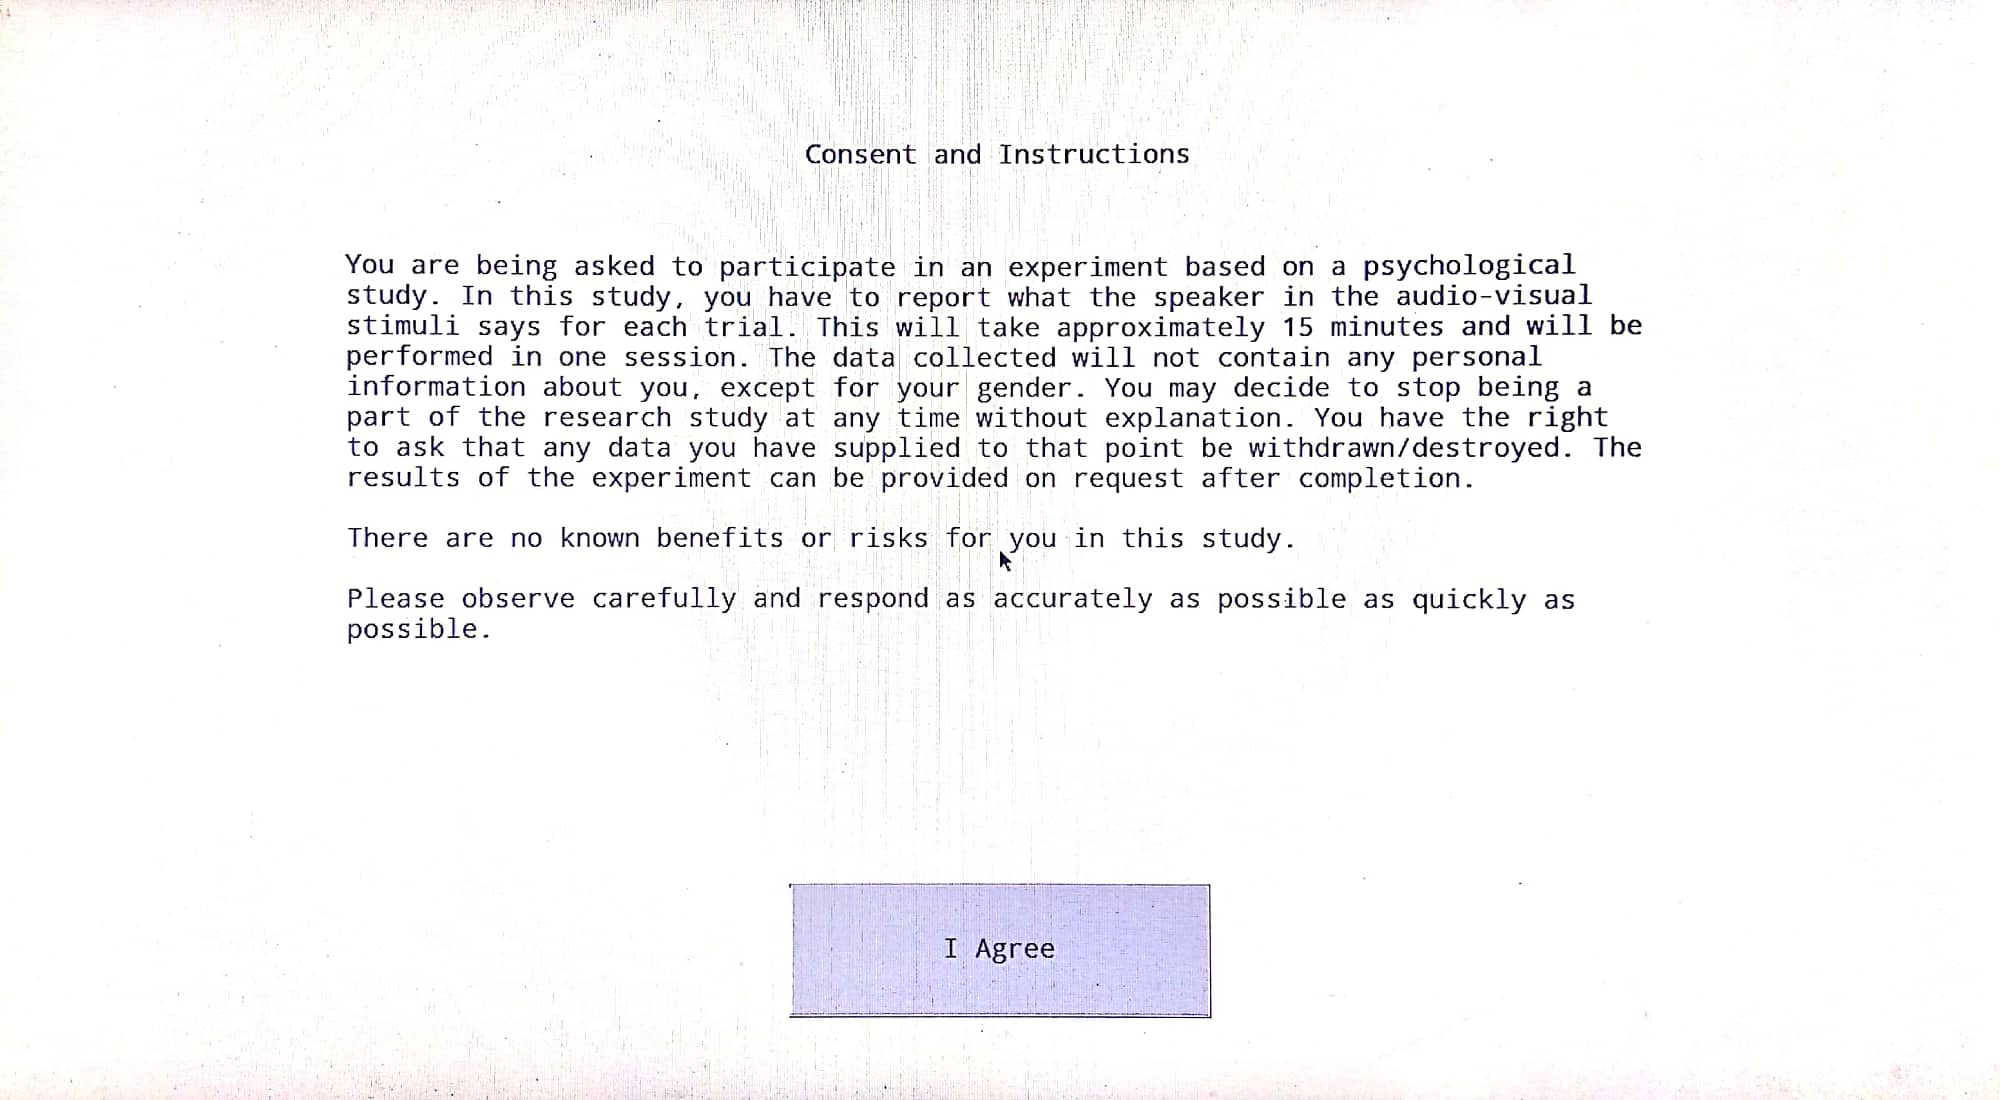
\includegraphics[width=1\textwidth]{includes/consent.jpg}
			\caption{Consent and Instructions Screenshot}
		\end{figure}

		`/ba/',`/pa/',`/ga/',`/va/',`/da/',`/ta/' and ``others". This was followed for all 45 trials and then "Thank you!" message was printed to indicate end of experiment.

		\begin{figure}[H]
			\centering
			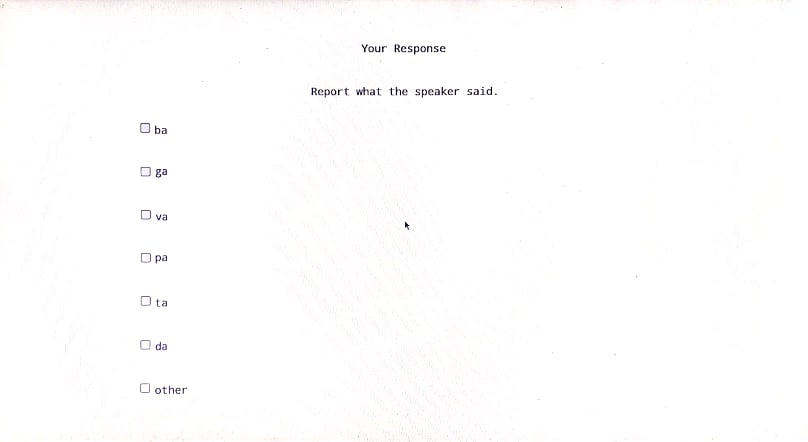
\includegraphics[width=1\textwidth]{includes/response.jpg}
			\caption{Response Form Screenshot}
		\end{figure}

	\end{psubsection}

\end{psection}

\begin{psection}{Data Analysis}

	\begin{psubsection}{Bias Removal}

		It is difficult to validate the visual influence as it is non-trivial to attribute an incorrect perception directly to incongruent visual information as there might be other factors affecting the listener's speech perceptiveness. In order to avoid this, as suggested by \cite{40-years}, we ought to add baseline unimodal conditions to ensure that illusory reports are explained by genuine integration mechanisms.

		A simple corrective method to minimize such biases in the collected data is to subtract the total number of fused responses by the number of auditory misidentifications for each subject \ie
		\begin{align*}
			\text{Illusory percepts = Fused percepts - Auditory Misidentifications}
		\end{align*}
		The auditory misidentifications, here, refer to the proportion of congruent responses that the listener misidentified.

	\end{psubsection}

	\begin{psubsection}{Data Visualization}
		After bias removal, a preliminary review of the collected data leads to the following bar chart. Visually influenced responses have been plotted for incoherent stimuli, i.e. audio '/ba' and video '/ga' or '/va'.

		\begin{figure}[H]
			\centering
			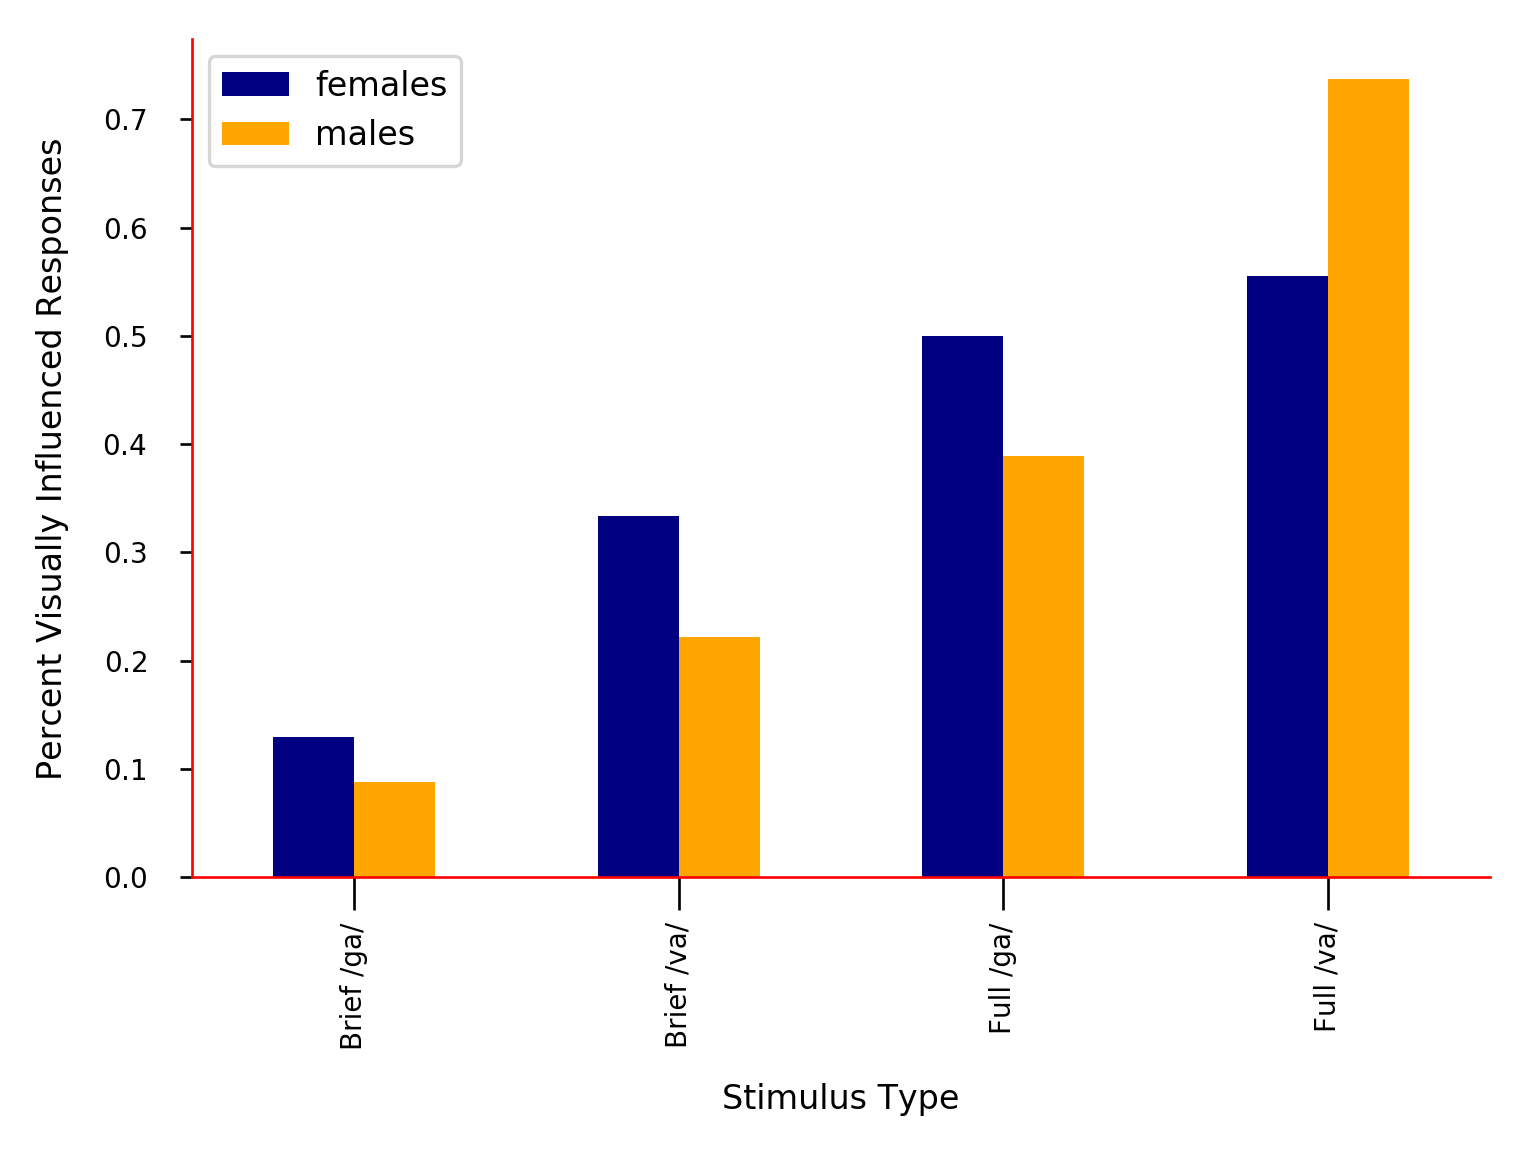
\includegraphics[width=0.8\textwidth]{includes/barchart.png}
			\caption{Visually Influenced Responses}
		\end{figure}

		Clearly, females seem to be more influenced as compared to males for the brief stimuli. However, no such clear statment can be made for tge full stimuli.

	\end{psubsection}

	\begin{psubsection}{ANOVA Analysis}

		ANOVA analysis is carried out, both, with and without bias removal. The recorded F-values and P-values follow.

		\begin{table}[H]
			\centering
			\begin{tabular}{|c|c|c|c|c|}
				\hline
				& \multicolumn{2}{c|}{\bt{Full Stimuli}} & \multicolumn{2}{c|}{\bt{Brief Stimuli}} \\
				\hline
				& \bt{F-Value} & \bt{p-value} & \bt{F-Value} & \bt{p-value} \\
				\hline
				\bt{Without Bias Removal} & 0.209 & 0.65 & 5.013 & 0.00158 \\
				\bt{With Bias Removal} & 0.766 & 0.387 & 2.457 & 0.126 \\
				\hline
			\end{tabular}
			\caption{Significance Values obtained using ANOVA Analysis}
			\label{tab:my_label}
		\end{table}

		Analyzing data after bias removal, p-value for brief stimuli suggests marginal significance while for the full stimuli suggests no significance. Hence, the difference in displaying McGurk effect between men and women is not significant in the case of full stimuli but marginally significant in the case of brief stimuli.

		\begin{table}[H]
			\centering
			\begin{tabular}{|c|c|c|}
				\hline
				&  \bt{Full Stimuli} & \bt{Brief Stimuli}\\
				\hline
				\bt{$\mu_M$}& $0.563$ & $0.135$\\
				\hline
				\bt{$\mu_F$}& $0.494$ & $0.219$\\
				\hline
			\end{tabular}
			\caption{Mean Values after Bias Removal}
			\label{tab:my_label}
		\end{table}

		Clearly, women show more McGurk effect than men in the case of brief stimuli with a p-value of 0.126.


	\end{psubsection}

\end{psection}

\begin{psection}{Result}
	In the study carried by Irwin and Whalen, influence of  gender was statistically marginal [F(1,64) = 3.11, p < 0.10] for brief stimuli. In our study, the result adhered to the observation, though not strictly, in the cited work as [F(1,35) = 2.457, p ~ 0.1] also showed the factor to be marginally significant. 
	\\For the experiment carried on full stimuli in Irwin’s study, the results were not significant which is in coherence with our observation of p-value = 0.387.


\end{psection}

\begin{psection}{Conclusion}
	As observed, perception of sound for women seems to be more visually influenced as compared to men in visually more difficult tasks(brief stimuli). It indicates the presence of difference of processing of audiovisual speech across genders which has been claimed in several studies; a more popular study states that lateralized processing of visual stimuli in female is more as compared to males which might contribute to observed and other difference in visual effects, an instance of which is the second experiment carried by Irwin and Whalen where they found women were able to perceive lip reading better for difficult tasks.
\end{psection}

\begin{thebibliography}{}
	\bibitem{original} Harry McGurk, John MacDonald: Hearing Lips and Seeing Voices [Nature]

	\bibitem{40-years}Agnès Alsius, Martin Paré and Kevin G. Munhall: Forty Years After Hearing Lips and Seeing Voices: the McGurk Effect Revisited https://doi.org/10.1163/22134808-00002565

	\bibitem{tribute}John MacDonald: Hearing Lips and Seeing Voices: the Origins and Development of the McGurk Effect and Reflections on Audio-Visual Speech Perception Over the Last 40 Years https://doi.org/10.1163/22134808-00002548

	\bibitem{sex difference}Irwin, J.R., Whalen, D.H. & Fowler, C.A. Perception & Psychophysics (2006) 68: 582 https://doi.org/10.3758/BF03208760

	\bibitem{model}John F. Magnotti, Michael S. Beauchamp, The Noisy Encoding of Disparity Model of the McGurk Effect (2015) https://www.ncbi.nlm.nih.gov/pmc/articles/PMC4370809/

\end{thebibliography}

\end{document}
